\documentclass[border=3mm]{standalone}

\usepackage{tikz}
\usetikzlibrary{arrows.meta,calc}

\begin{document}
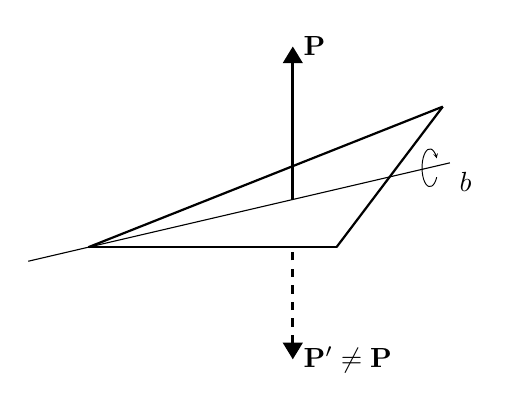
\begin{tikzpicture}[scale=0.75]
\newcommand{\AxisRotator}[1][rotate=0]{%
    \tikz [x=0.25cm,y=0.60cm,line width=.2ex,-stealth,#1] \draw (0,0) arc (-150:150:1 and 1);%
}
\draw[very thick,dashed,Triangle-] (-2.94,-3.5) node[right] {$\mathbf{P'}\neq \mathbf{P}$} -- (-2.94,-0.8);
\fill[white] (-6.4,-1.6) -- (-2.2,-1.6) -- (-0.4,0.78) -- cycle;
\draw[thick] (-6.4,-1.6) coordinate (1)  -- (-2.2,-1.6);
\draw[thick] (-2.2,-1.6) -- (-0.4,0.78) coordinate[pos=0.5](2);
\draw[thick] (-0.4,0.78) -- (-6.4,-1.6);
\draw[very thick,-Triangle] (-2.94,-0.8) -- (-2.94,1.8) node[right] {$\mathbf{P}$};
\draw ($(1)!-.2!(2)$) -- ($(2)!-.2!(1)$) node[pos=0.95,scale=0.4,xscale=-1]{\AxisRotator} node[below right] {$b$};
\end{tikzpicture}
\end{document}